\chapter{Neurónové siete}


Neurónová sieť je založená na orientovanom grafe (ako je možné vidieť na obrázku \ref{fig:nn}), je teda zložená z uzlov, ktoré sú spojené orientovanými hranami \citep{rnn:spol}.
Spojenie uzlu $i$ do uzlu $j$ slúži na propagáciu aktivácie $a_i$ z $i$ do $j$.
Každé takéto spojenie má priradenú váhu $w_{i,j}$, ktorá rozhoduje o sile a znamienku spojenia.
Každý uzol má naviac falošný vstup $a_0=1$ s priradenou váhou $w_{0,j}$.
Všetky uzly si potom vypočítajú váženú hodnotu vstupov, pre uzol $j$ je táto hodnota:
$$in_j=\sum^n_{i=0}w_{i,j}a_i$$
Potom sa na výsledok aplikuje aktivačná funkcia g, tým získame výstup z uzlu:
$$a_j=g(in_j)=g\left(\sum^n_{i=0}w_{i,j}a_i\right)$$

\begin{figure} \label{fig:nn}
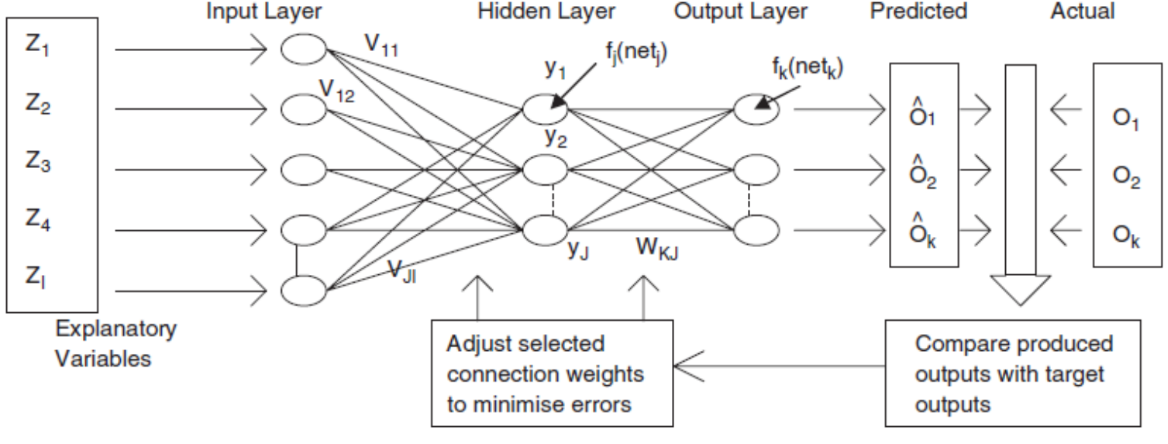
\includegraphics[width=\textwidth]{../img/nn.png}
\caption{Ukážka jednej z neurónových sietí}
\end{figure}

Aktivačná funkcia $g$ je typicky buď pevná hranica alebo logistická funkcia.
V prvom prípade sa uzly volajú perceptrony, v druhom prípade sa niekedy používa pojem sigmoid perceptron.
Obe tieto typy nelineárnych aktivačných funkcií zaručujú dôležitú vlastnosť neurónovej siete, a to, že celá sieť uzlov môže reprezentovať aj nelineárnu funkciu.

\begin{figure}
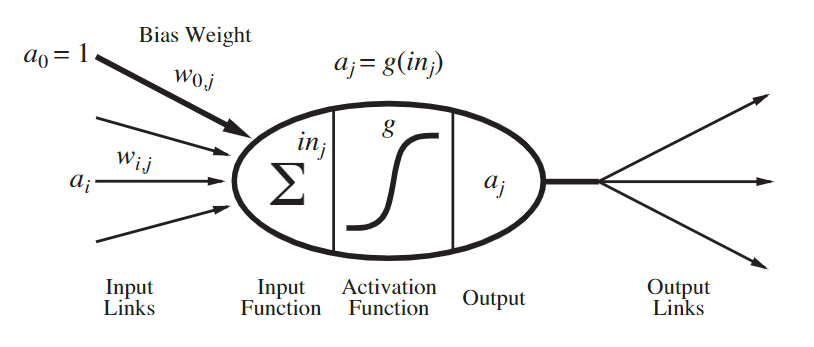
\includegraphics[width=\textwidth]{../img/nn_aima_neuron.png}
\caption{Takto vyzerá jeden uzol siete (neurón) \citep{aima}.}
\end{figure}

Takto teda vyzerá matematický model jedného uzlu (v tomto prípade zvaného neurón) v sieti.
Spájanie týchto neurónov vytvorí sieť.
Existujú dva rozdielne prístupy, akými sa dajú tieto neuróny spojiť do siete. 
Obe nás zaujímajú pre túto prácu, pretože obe použijeme v praxi a budeme ich porovnávať medzi sebou. Tieto dva prístupy tvoria doprednú, respektíve rekuretnú neurónová sieť.

\section{Dopredné neurónové siete}
Dopredná neurónová sieť (feed-forward neural network \citep{aima}) má spojenia len v jednom smere, takže tvorí orientovaný acyklický graf (obrázok \ref{fig:nn} zobrazuje práve tento typ siete).
Ak si graf topologicky usporiadame, tak každý uzol dostane vstup z niektorých z predchádzajúcich uzlov a predá výstup niektorým z nasledujúcich vrcholov.
Dopredná neurónová sieť teda predstavuje funkciu jej momentálneho vstupu, teda neuchováva žiaden stav, ak nepočítame váhy samotné.

Tieto siete sú obvykle zoradené do vstiev tak, že každý neurón dostane vstup len z neurónov z predošlej vrstvy.
Podľa počtu vrstiev sa siete delia na jednovrstvové a viacvrstvové .

\subsection{Jednovrstvové siete}
Jednovrstvové siete spájajú vstupné neuróny priamo s výstupnými.
Tieto siete sú ale obmedzené a nevedia sa naučiť funkcie, ktoré nie sú lineárne separabilné, platí to dokonca aj pre niektoré jednoduché funkcie ako napríklad XOR \citep{aima}. 

V Euklidovskej geometrii je lineárna separabilita vlastnosť dvoch množín bodov v priestore, ktoré sa dajú presne oddeliť nadrovinou v tomto priestore. 
Najjednoduchšie sa to dá predstaviť v dvojrozmernom priestore napríklad na boolovskej funkcii OR. Bodu (0,0) v súradnicovom systéme (x,y) priradí funkcia hodnotu 0, bodom (1,0), (0,1) a (1,1) priradí hodnotu 1. Ak body rozdelíme do množín podľa priradenej hodnoty, tak tieto dva množiny sa dajú presne oddeliť priamkou, napríklad $y = -x + 1/2$. Je zjavné, že množiny bodov získané z funkcie XOR (tabuľka \ref{xor}) sa takto rozdeliť nedajú, tieto množiny teda nie sú lineárne separabilné.

\begin{table}[h]
\begin{center}
\begin{tabular}{ |c|c|c| } 
 \hline 
 x & y & x XOR y \\ 
 \hline
 0 & 0 & 0 \\ 
 0 & 1 & 1 \\ 
 1 & 0 & 1 \\ 
 1 & 1 & 0 \\ 
 \hline
\end{tabular}
\caption{Tabuľka funkcie XOR}
\label{xor}
\end{center}
\end{table}

\subsection{Viacvrstvové siete}
Viacvrstvové siete majú medzi vstupom do siete a výstupom z nej ešte jednu alebo viac vrstiev tzv. skrytých (hidden) neurónov (Obrázok \ref{img:single}).
Waren McCulloch a Walter Pitts vo svojom článku dokázali, že jeden neurón v sieti vie reprezentovať základné boolovské funkcie AND, OR a NOT a vyslovili, že každá dodatočná funkcionalita sa dá získať spojením väčšieho počtu neurónov do siete \citep{multi}. Samotné XOR z predchádzajúcej podsekcie sa dá vyjadriť ako 
\textit{(x OR y) AND (NOT(x) OR NOT(y))} a podľa tohto vieme vytvoriť aj jednoduchú viacvrstvovú sieť, ktorá používa len neuróny s funkciami AND, OR a NOT (obrázok \ref{img:xor}, matematika týchto viacvrstvových modelov nám však dovoľuje vytvoriť aj jednoduchšie siete pre rozoznávanie XOR, je len potrebné zmeniť aktivačnú funkciu a váhy jednotlivých spojení).

\begin{figure} \label{img:single}
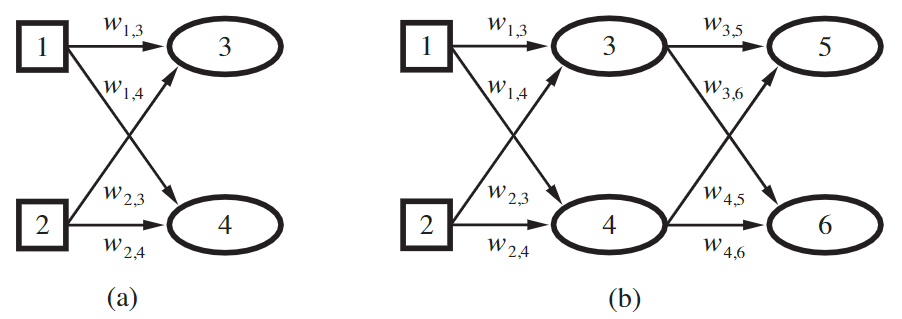
\includegraphics[width=\textwidth]{../img/nn_aima_single_multi.png}
\caption{Ukážka rozdielu medzi jednovrstvou sieťou (a) a viacvrstvovou (b). Obe majú 2 vstupné a 2 výstupné neuróny, viacvrstvová má ešte medzi nimi ďalšie vrstvy skrytých neurónov (v tomto prípade jednu vrstvu s 2 skrytými neurónmi), falošné vstupy do každého neuŕony nie sú ukázané \citep{aima}.}
\end{figure}

\begin{figure} \label{img:xor}
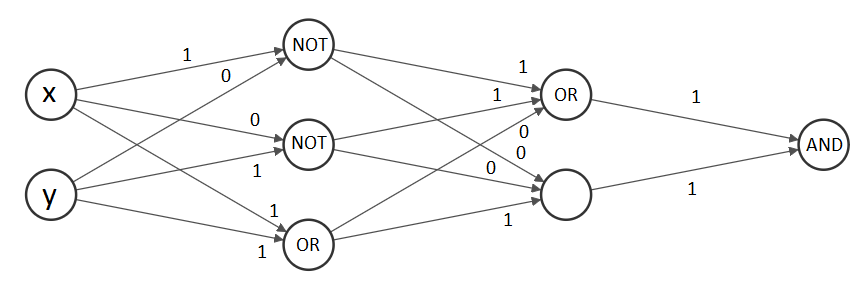
\includegraphics[width=\textwidth]{../img/xor.png}
\caption{Jednoduchá ukážka viacvrstvovej neurónovej siete rozoznávajúcej XOR.}
\end{figure}


\section{Rekurentné neurónové siete}
Na druhej strane je rekurentná neurónová sieť (recurrent neural network).
Tento typ siete posúva svoj výstup naspäť do svojho vlastného vstupu. 
Z toho vyplýva, že aktivačné úrovne siete tvoria dynamický systém, ktorý môže dosiahnuť stabilný stav alebo oscilovať či sa dokonca správať chaoticky.

Výstup siete závisí na vstupe. 
Pri tomto type siete môže výstup závisieť aj na predchádzajúcich výstupoch, tranzitívne teda aj na predchádzajúcich vstupoch.
Z toho vyplýva, že si rekurentná neurónová sieť môže vypracovať krátkodobú pamäť \citep{aima}.

\section{Učenie}
V predchádzajúcich sekciách sme hovorili o nastavení váh jednotlivých spojení medzi neurónmi a výbere aktivačnej funkcie.
V praxi si ale tieto hodnoty obvykle nenastavujeme manuálne, ale nastavuje si ich sieť sama procesom zvaným učenie. Neurónová sieť je učená iteratívnym spôsobom. 
V každej iterácii dostane sieť množinu vstupov.
Pre každý vstup vypočíta hodnotu odhadovaného výstupu, potom sa sieť pozrie na očakávaný výstup a zapamätá si rozdiel týchto hondôt.
Po skončení iterácie sa sieť pozrie na hodnoty týchto rozdielov a upraví si svoje váhy tak, aby nabudúce pri rovnakých datach vydala výstup bližší k očakávanému výstupu.
Proces by mal naučiť sieť ohodnotiť celý dataset čo najpresnejšie.
Ak data dobre reprezentujú celý problém a nie len nejakú jeho časť, tak sa môže naučiť generalizovať, teda vydať správny výstup aj na data, ktoré predtým nikde nevidela.

Konkrétnejšie, začneme v procese učenia inicializáciou váh. Tie sa obvykle inicializujú náhodne.
Po inicializácii začne už spomínaný iteratívny proces.
V každom kroku zvolíme príslušnú podmnožinu trénovacích dat (v angličtine \textit{batch}) a vyhodnotíme vypočítané výstupy porovnaním s očakávanými a pozmeníme jednotlivé váhy podľa toho.
Vypočítané výstupy sa vyhodnocujú pomocou stratovej funkcie.
Našou úlohou je hodnoty stratovej funkcie minimalizovať.
Jednou z najpoužívanejších stratových funkcií je stredná štvorcová chyba (v angličine \textit{Mean Squared Error}). Táto funkcia je definovaná ako funkcia $$MSE(x,y,f) = \frac{1}{m} \cdot \sum_{i=1}^m (f(x)_i - y_i)^2$$
kde
$f: \mathbb{R}^n \to \mathbb{R}^m$ je funkcia, ktorú simuluje neurónová sieť, $x \in \mathbb{R}^n$ vstupný vektor a $y \in \mathbb{R}^m$ očakávaná hodnota výstupu.
To je hodnota MSE pre jeden vstup, ale my trénujeme v podmnožinách vstupných dat veľkosti $k$ a až potom vyhodnocujeme. 
Pre tento prístup je MSE definovaná $$MSE(X,Y,f) = \frac{1}{k} \cdot \sum_{j=1}^k (MSE(X_j,Y_j,f)) = \frac{1}{k} \cdot \sum_{j=1}^k (\frac{1}{m} \cdot \sum_{i=1}^m  (f(X_j)_i - Y_{j_i})^2)) $$
kde $X \in \mathbb{R}^k \times \mathbb{R}^n$ je množina vstupných vektorov a $Y \in \mathbb{R}^k \times \mathbb{R}^m$ je množina očakávaných výstupov.

Na riešenie klasifikačných problémov, teda problémov, kde výstupom je vektor, ktorý obsahuje samé 0 a jednu 1, ktorá určuje, do ktorej triedy je vstup zaradený (ako v našom prípade, kde klasifikujeme zápasy na výhry, prehry a v prípade futbalu aj remízy), sa používa softmaxová strata.
Softmaxová strata (niekde v literatúre aj cross-entropy loss) sa aplikuje len, keď je aktivačná funkcia vo výstupných neurónoch softmax ($\sigma: \mathbb{R}^k \to \mathbb{R}^k$ daná ako $\sigma(z)_i = \frac{e^{z_i}}{\sum_{j=1}^k e^{z_j}}$).
Vlastnosti tejto funkcie ukazujú, že súčet všetkých zložiek výstupného vektora je 1, takže táto funkcia v prípade neurónových funkcií ukazuje názor siete na to, ako pravdepodobné je, že sa vstup nachádza v triede $i \forall i \in {1,\dots , k}$.
Na konci sa vždy upraví výstup softmaxu tak, aby bol výsledný vektor vhodný výstupu (teda najvyššia hodnota sa premení na 1, zvyšné na 0). Označme si tento výstupný vektor ako $v$.
Keď je súčet zložiek rovný 1, vieme použiť funkciu na výpočet entropie ($ H = -\sum_{i=1}^k \left(x_i \cdot log_2(x_i)\right) $).
Takže softmaxová stratová funkcia vyzerá nasledovne ($p \in {1,\dots ,k}$ je $argmax_{\sigma(z)}$)
$$L(x,y) = -\sum_{i=1}^k \left(v_i*log_2(\sigma(z)_i)\right) = -\sum_{i=1}^k log_2\left(\frac{e^{z_p}}{\sum_{j=1}^k e^{z_{j}}}\right)  $$

Ďalšie masívne používané stratové funkcie sú 
absolútna strata ($L(x,y,f) = $ $\frac{1}{m}\sum_{i=1}^m \left|f(x)_i - y_i\right|$), 
$\epsilon$-necitlivá strata ($L(x,y,f) = \frac{1}{m}\sum_{i=1}^m \left(\left|f(x)_i - y_i\right| - \epsilon\right)$), 
logistická strata ($L(x,y,f) = \frac{1}{m} \sum_{i=1}^m  \left((ln(2))^{-1}\cdot ln(1+e^{-f(x)_iy_i})\right) $).
\citep{loss}.

Jedným zo spôsobov, ktoré sa používajú na úpravu jednotlivých váh je tzv. \textit{Gradient descent}.
Matematická analýza nám umožňuje získať smer stúpania každej diferencovateľnej funkcie.
Prirodzene, hodnoty stratovej funkcie sa snažíme znížiť, teda posunúť váhy v smere klesania, teda proti smeru stúpania stratovej funkcie.
Na to potrebujeme diferencovateľnú stratovú funkciu, z čoho vyplýva, že aj neurónová sieť a aktivačné funkcie vo vnútri, musia byť diferencovateľné.
Naším cieľom je vypočítať gradient stratovej funkcie.
Keď ho nájdeme, zameníme v ňom znamienka, teda prenásobíme ho číslom $-1$.
Následne môžeme v tomto smere zmeniť váhy.
Váhy sa menia v čase $t$ nasledovne: 
$$w_{t+1} = w_t - \alpha \cdot \frac{1}{n} \sum_{i=1}^n \nabla_w L(x,y,f_t)$$
kde $L$ je stratová funkcia, $f_t$ je funkcia, ktorú neurónová sieť simuluje v čase $t$  a $\alpha \in \mathbb{R}^+$ je veľkosť modifikácie (v angličtine \textit{learning rate}) a jeho hodnoty sa môžu podľa algoritmu učenia meniť počtom iterácií \citep{nn:gd}. Veľkosť modifikácie by sme ideálne chceli malú, aby sme náhodou minimum stratovej funkcie nepreskočili. Ak je ale veľkosť modifikácie príliš nízka, učenie trvá dlho.

O trochu zložitejším spôsobom je \textit{Adam} \citep{adam}.
Názov je vytvorený zo súslovia adaptívny odhad momentu (v angličtine \textit{ADAptive Moment estimation}).
Tento spôsob funguje na podobnom princípe ako Gradient Descent s výnimkou toho, že si pamätá a používa pár posledných gradientov, ich význam postupne znižuje.
V situácii, kde Gradient Descent narazí za lokálne minimum, algoritmus začne meniť váhy v opačnom smere, zatiaľ čo Adam bude ešte jemne posúvať algoritmus v smere, v ktorom išiel predtým a možno sa stane, že prekoná lokálne maximum a opäť pôjde smerom dole (ukážku vidieť na obrázku \ref{adam}). Ak sa nedostane cez lokálne maximum, tak sa eventuálne uspokojí a skončí na rovnakom mieste, ako by skončil Gradient Descent.
\noindent
\begin{figure} \label{adam}
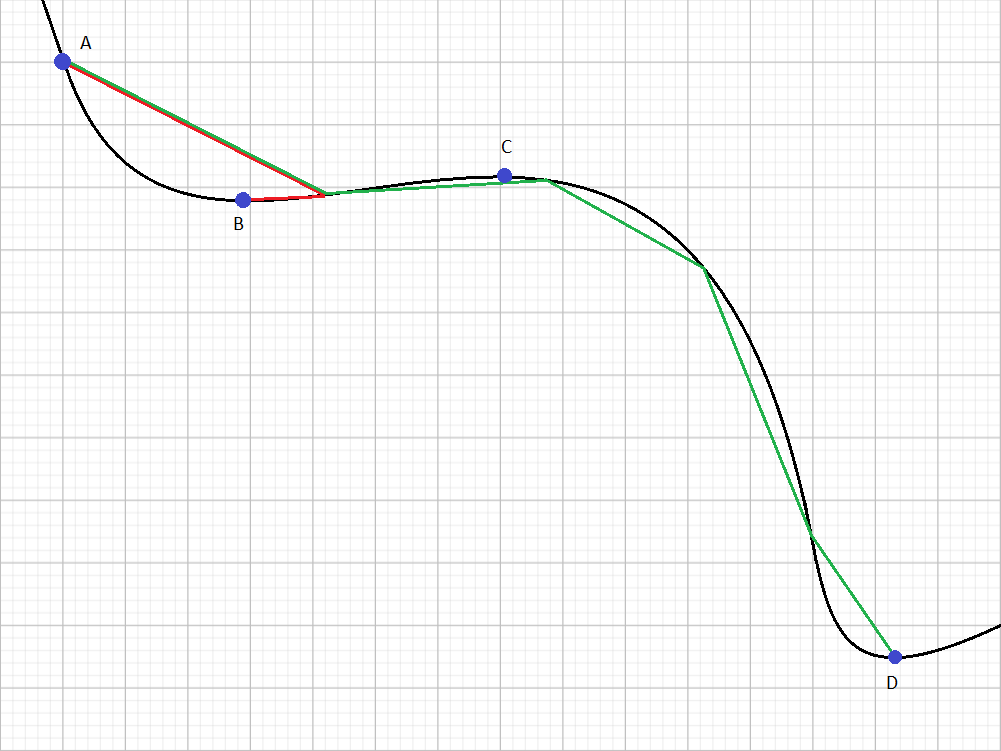
\includegraphics[width=\textwidth]{../img/gd_adam.png}
\caption{Ukážka rozdielu medzi algoritmami Gradient Descent (červenou) a Adam (zelenou). Čiernou farbou je znázornený graf hodnôt nejakej stratovej funkcie, A je bod, na ktorom obe algoritmy začínajú, B je lokálne minimum, C lokálne maximum a D globálne minimum. Adam používa aj gradienty z minulých iterácií a tak je schopný preskočiť lokálne maximum a pokračovať ďalej.}
\end{figure}

Jedným z problémov neurónových sietí je to, že dosiahnuť ani len lokálne minimum nemusí byť požadujúce.
Ideálne požadujeme, aby sieť správne generalizovala, a teda aby jej výstup bol správny aj pre data, na ktorých sa neučila.
Aj keď trénovacia vzorka reprezentatuje realitu, môže sa stať, že sieť bude mať nízku hodnotu trénovacej chyby (stratovej funkcie), ale relatívne vysokú hodnotu testovacej chyby (príklad možno vidieť na obrázku \ref{overf}). Testovacia chyba sa vypočítava ako hodnota používanej stratovej funkcie na datach, ktoré neboli obsiahnuté v trénovacej vzorke.
Tomuto fenoménu sa hovorí pretrénovanie (v angličtine \textit{overfitting}) \citep{overfit}.

\noindent
\begin{figure} \label{overf}
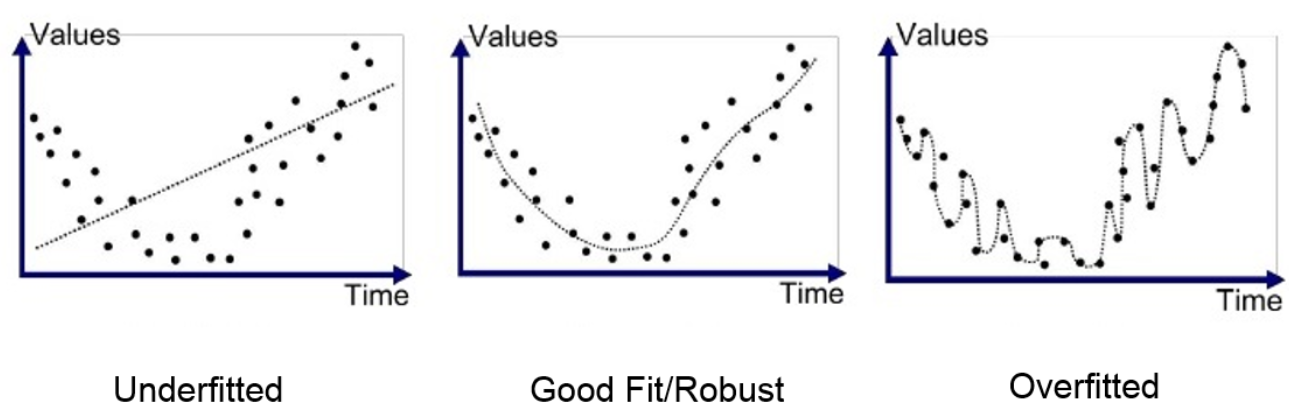
\includegraphics[width=\textwidth]{../img/overfit.png} 
\caption{Ukážka troch stavov, v ktorých sa môže sieť nachádzať: môže byť podtrénovaná (underfitted), správne natrénovaná (good fit) a pretrénovaná (overfitted) \citep{gitgud}.}
\end{figure}